\paragraph{}Esta es la página principal o de inicio de la aplicación web $\mu$Search.

\paragraph{}Se le muestra al usuario un mensaje de bienvenida y una breve descripción de en que consiste la página web $\mu$Search, de la empresa creadora y de que se ofrece a través del catálogo electronico.

\begin{figure}[h!]
	\centering
	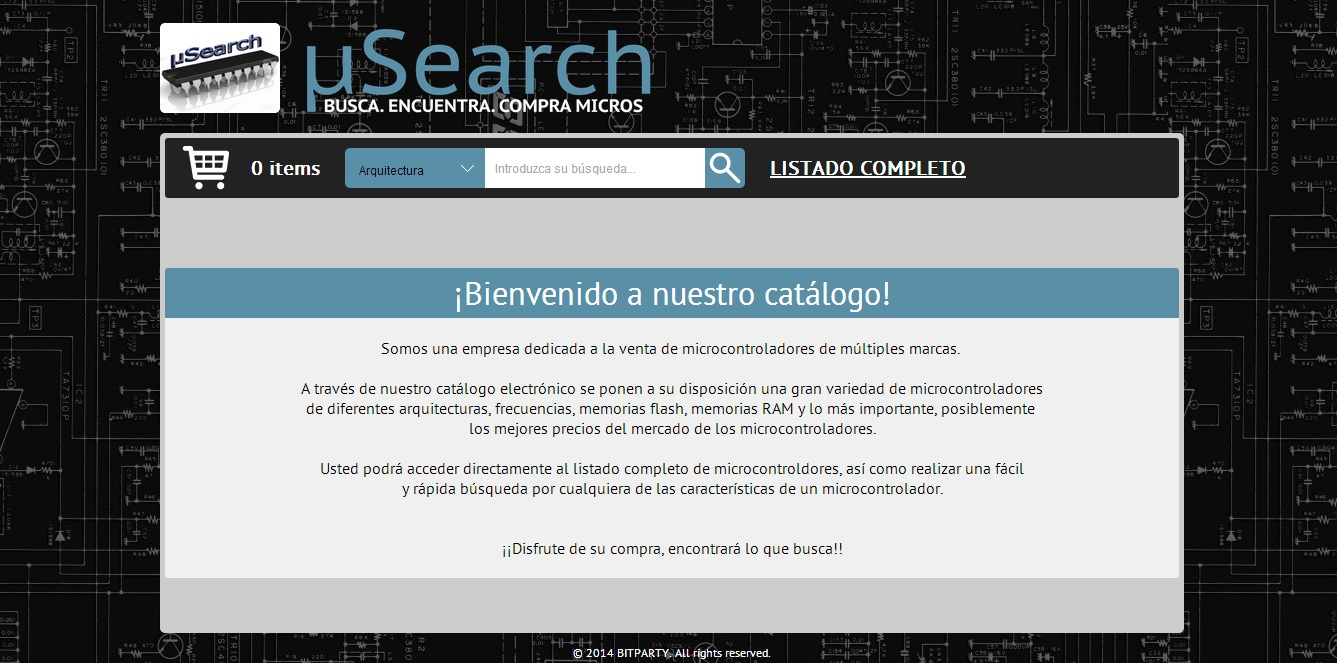
\includegraphics[width=0.85\textwidth]{img/principal_user}
	\caption{Página principal de usuario.}
	\label{fig:principal_usuario}
\end{figure}

Desde esta página, a través de los iconos situados en la cabecera debajo de los logotipos de la web, el usuario puede acceder a:
\begin{itemize}
	\item\textbf{Carrito de la compra:} Redirige al usuario a la página del carrito de la compra.
	
	\item \textbf{Búsqueda:} Desde esta sección, el usuario puede realizar búsquedas sobre el catálogo de microcontroladores en base a cualquiera de sus características (Arquitectura, Frecuencia, Flash, RAM). Se debe seleccionar una de las características de la lista despegable, introducir el texto a buscar y pulsar sobre el icono de búsqueda.
	El usuario será redirigido a una página donde se le mostrará el resultado de la búsqueda.
	
	\item \textbf{Listado Completo:} Redirige al usuario a la página en la que se listan todos los microcontroladores disponibles en el catálogo.
	
\end{itemize}